\PassOptionsToPackage{dvipsnames}{xcolor}
\documentclass[border=3mm]{standalone}
\usepackage{pgfplots}
\usepgfplotslibrary{groupplots}
\pgfplotsset{compat=1.17}
\usepackage[dvipsnames]{xcolor}
\usepackage{amsmath}
\usepackage{amssymb}
\usepackage{relsize}

\newcommand{\Tukeywindow}[3]{% beta, delay, color
\addplot[#3, domain=#2-(1+#1)/2:#2+(1+#1)/2, samples=100, thick] {func(x-#2,#1)};
}


\tikzset{fontscale/.style = {font=\relsize{#1}}
    }

\begin{document}

\pgfplotsset{
compat=1.11,
legend image code/.code={
\draw[mark repeat=2,mark phase=2]
plot coordinates {
(0cm,0cm)
(0.15cm,0cm)        %% default is (0.3cm,0cm)
(0.3cm,0cm)         %% default is (0.6cm,0cm)
};%
}
}

\definecolor{lightblue}{RGB}{86,192,150}  % Define light blue color

\pgfdeclarelayer{background layer}
\pgfdeclarelayer{foreground layer}
\pgfsetlayers{background layer,main,foreground layer}

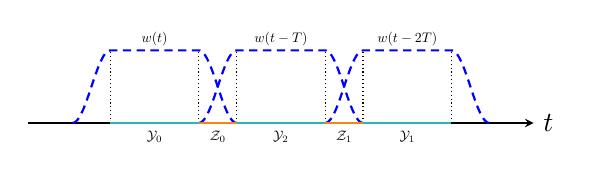
\begin{tikzpicture}[
declare function={
	func(\x,\b)= and(\x >= -(1-\b)/2, \x<= (1-\b)/2) * 2/sqrt(4-\b) + 
		       and(\x >= -(1+\b)/2, \x <= -(1-\b)/2) * 1/sqrt(4-\b)*(1+sin(deg(pi*(2*\x+1)/(2*\b)))) +
		       and(\x >= (1-\b)/2, \x <= (1+\b)/2) * 1/sqrt(4-\b)*(1-sin(deg(pi*(2*\x-1)/(2*\b)))) ;		       
},
]
\begin{axis}[
  width = 8cm,
  height = 3cm,
  xlabel={$t$},
  axis x line=middle,  % Show only the x-axis
  axis y line=none,    % Hide the y-axis
  xmin=-2, xmax=2,
  ymin=-0.1, ymax=1.5,  % Set ymax to 2
  xtick=\empty,
  ytick=\empty,
  every tick label/.append style={scale=0.5},
  xlabel style={
    right,
  },
  legend style={draw=none,nodes={scale=0.4, transform shape}}
]

\Tukeywindow{0.3}{-1}{blue,densely dashed}
\Tukeywindow{0.3}{0}{blue,densely dashed}
\Tukeywindow{0.3}{1}{blue,densely dashed}
\addplot [black, densely dotted] coordinates {(-1.35,0)(-1.35,1.0397504898)};
\addplot [black, densely dotted] coordinates {(-0.65,0)(-0.65,1.0397504898)};
\addplot [black, densely dotted] coordinates {(-0.35,0)(-0.35,1.0397504898)};
\addplot [black, densely dotted] coordinates {(0.35,0)(0.35,1.0397504898)};
\addplot [black, densely dotted] coordinates {(0.65,0)(0.65,1.0397504898)};
\addplot [black, densely dotted] coordinates {(1.35,0)(1.35,1.0397504898)};

\addplot [BlueGreen, thick] coordinates {(-1.35,0)(-0.65,0)};
\addplot [BlueGreen, thick] coordinates {(-.35,0)(0.35,0)};
\addplot [BlueGreen, thick] coordinates {(0.65,0)(1.35,0)};

\addplot [BurntOrange, thick] coordinates {(-0.65,0)(-0.35,0)};
\addplot [BurntOrange, thick] coordinates {(0.35,0)(0.65,0)};

\coordinate (s0) at (axis cs: -1,1.2);
\coordinate (s1) at (axis cs: 0,1.2);
\coordinate (s2) at (axis cs: 1,1.2);

\coordinate (y0) at (axis cs: -1,-0.2);
\coordinate (y1) at (axis cs: 0,-0.2);
\coordinate (y2) at (axis cs: 1,-0.2);

\coordinate (z0) at (axis cs: -0.5,-0.2);
\coordinate (z1) at (axis cs: 0.5,-0.2);


\end{axis}

\node [style={scale=0.5}] at (s0) {$w(t)$};
\node [style={scale=0.5}] at (s1) {$w(t-T)$};
\node [style={scale=0.5}] at (s2) {$w(t-2T)$};

\node [style={scale=0.5}] at (y0) {$\mathcal{Y}_0$};
\node [style={scale=0.5}] at (y1) {$\mathcal{Y}_2$};
\node [style={scale=0.5}] at (y2) {$\mathcal{Y}_1$};

\node [style={scale=0.5}] at (z0) {$\mathcal{Z}_0$};
\node [style={scale=0.5}] at (z1) {$\mathcal{Z}_1$};

\end{tikzpicture}

\end{document}
























